\documentclass[stu, 12pt, letterpaper, donotrepeattitle]{apa7}
\usepackage[utf8]{inputenc}
\usepackage[spanish]{babel}
\usepackage{csquotes}
\usepackage{hyperref}
\usepackage{graphicx}



% Configuración de hipervínculos para APA
\hypersetup{colorlinks=true, allcolors=black}

%----------------------------------------------------------------------------------------
%	METADATOS DE PORTADA (APA 7)
%----------------------------------------------------------------------------------------

% Título del reporte
\title{Avance de Proyecto: Diseño y Análisis}

% Nombre del estudiante
\author{Fernando Israel Rios Garcia-AL02877016} 

% Afiliación (Departamento y Universidad)
\affiliation{Universidad Tecmilenio-Campus Corregidora} 

% Código y nombre del curso
\course{LSTI2307: Programación Orientada a Objetos}

% Nombre del instructor/profesor
\professor{Ricardo Monrroy}

% Fecha de entrega
\duedate{\today}

%----------------------------------------------------------------------------------------

\begin{document}

    % Genera la portada APA 7 automáticamente
    \maketitle

    %----------------------------------------------------------------------------------------
    %	CONTENIDO DEL REPORTE
    %----------------------------------------------------------------------------------------

    \section{Análisis de Requerimientos}
    
    \subsection{Objetivo}
    El sistema busca eficientizar y automatizar la gestión administrativa de una biblioteca mediante una solución de software desarrollada en Java. El objetivo principal es facilitar el registro y consulta de libros, usuarios y préstamos, asegurando la integridad de los datos a través de validaciones robustas y reglas de negocio, como el control de stock y límites de préstamo por usuario. Asimismo, el sistema está diseñado para proveer reportes claros sobre el estado operativo de la biblioteca, priorizando la facilidad de uso, eficiencia y una arquitectura escalable que permita futuras expansiones, todo ello en cumplimiento con los lineamientos académicos de la materia LSTI2307.

    \subsection{Requisitos Funcionales}
    El sistema cumple con las siguientes funciones esenciales:
    \begin{itemize}
        \item \textbf{Gestión de Entidades}: Registro y consulta de libros, usuarios y préstamos.
        \item \textbf{Validación de Datos}: Verificación de coherencia y corrección en la información ingresada.
        \item \textbf{Reglas de Negocio}: Control de stock (no prestar libros sin disponibilidad) y límite de préstamos (máximo dos ejemplares por usuario).
        \item \textbf{Reportes}: Generación de informes en pantalla sobre el estado general de la biblioteca, incluyendo conteos de libros, usuarios y préstamos activos.
    \end{itemize}

    \section{Diseño de Clases y Objetos}

    A continuación se detallan las clases principales identificadas en el modelo orientado a objetos, las cuales representan las entidades fundamentales del dominio de la biblioteca.

    \subsection{Clase Principal}
    \begin{description}
        \item[Library] Actúa como el controlador principal del sistema.
        \begin{itemize}
            \item \textbf{Atributos}: Listas de usuarios (\texttt{users}), materiales (\texttt{materials}), mobiliario (\texttt{furniture}) y préstamos (\texttt{loans}).
            \item \textbf{Métodos}: Permite registrar usuarios, materiales y préstamos (\texttt{registerUser}, \texttt{registerLoan}), así como generar reportes generales (\texttt{generateReport}).
        \end{itemize}
    \end{description}

    \subsection{Entidad Base}
    \begin{description}
        \item[LibraryEntity (Abstracta)] Clase base para todos los objetos gestionables en la biblioteca.
        \begin{itemize}
            \item \textbf{Atributos}: Identificador (\texttt{id}), nombre (\texttt{name}) y fecha de creación (\texttt{createdAt}).
            \item \textbf{Métodos}: Validación básica de la entidad (\texttt{validate}).
        \end{itemize}
    \end{description}

    \subsection{Jerarquía de Usuarios}
    Heredan de \texttt{LibraryEntity}.
    \begin{description}
        \item[User] Representa a un usuario genérico.
        \begin{itemize}
            \item \textbf{Atributos}: Apellidos, edad, email, balance y préstamos activos.
            \item \textbf{Métodos}: Verificar elegibilidad (\texttt{canBorrow}), agregar o remover préstamos.
        \end{itemize}
        \item[Visitor] Subclase de Usuario. Tiene un límite de préstamos predefinido (e.g., 2 ítems).
        \item[Librarian] Subclase de Usuario. Posee un rol administrativo y métodos para registrar libros y usuarios en el sistema.
    \end{description}

    \subsection{Jerarquía de Materiales}
    Heredan de \texttt{LibraryEntity}.
    \begin{description}
        \item[Material] Clase base para los recursos prestables.
        \begin{itemize}
            \item \textbf{Atributos}: Autor, fecha de publicación, stock y condición.
            \item \textbf{Métodos}: Verificación de disponibilidad (\texttt{isAvailable}) y gestión de stock.
        \end{itemize}
        \item[Book] Atributos específicos: ISBN, editorial, categoría en estante.
        \item[Magazine] Atributos específicos: Volumen, número.
        \item[DVD] Atributos específicos: Duración, región.
    \end{description}

    \subsection{Jerarquía de Mobiliario}
    Heredan de \texttt{LibraryEntity}.
    \begin{description}
        \item[Furniture] Clase base para el inventario físico no prestable.
        \begin{itemize}
            \item \textbf{Atributos}: Fecha de ingreso y estado operativo (\texttt{isOperational}).
        \end{itemize}
        \item[Shelf] Estantería. Define capacidad y sección.
        \item[Desk] Escritorio. Define capacidad de asientos y ubicación.
        \item[Chair] Silla. Define material, si es ergonómica y si tiene ruedas.
    \end{description}

    \subsection{Gestión de Préstamos}
    \begin{description}
        \item[Loan] Modela la transacción de préstamo.
        \begin{itemize}
            \item \textbf{Atributos}: Fecha de inicio, fecha de vencimiento y estado.
            \item \textbf{Métodos}: Cerrar préstamo (\texttt{closeLoan}) y verificar si está vencido (\texttt{isOverdue}).
        \end{itemize}
    \end{description}

    \section{Relación entre Clases}

    La arquitectura del sistema se basa en las siguientes relaciones estructurales:

    \subsection{Herencia (Generalización)}
    Se ha implementado una jerarquía robusta para reutilizar código y agrupar comportamientos comunes:
    \begin{itemize}
        \item \textbf{LibraryEntity} es la clase padre de \texttt{User}, \texttt{Material} y \texttt{Furniture}. Esto permite que todas las entidades compartan propiedades básicas como ID y fecha de registro.
        \item \textbf{User} es padre de \texttt{Visitor} y \texttt{Librarian}.
        \item \textbf{Material} es padre de \texttt{Book}, \texttt{Magazine} y \texttt{DVD}.
        \item \textbf{Furniture} es padre de \texttt{Shelf}, \texttt{Desk} y \texttt{Chair}.
    \end{itemize}

    \subsection{Composición (Todo-Parte)}
    La clase \textbf{Library} mantiene una relación de composición fuerte con las entidades del sistema. La biblioteca "posee" las listas de usuarios, materiales, muebles y préstamos. Si la biblioteca dejara de existir, el contexto de estas colecciones desaparecería.
    \begin{itemize}
        \item \texttt{Library "1" *-- "*" LibraryEntity}
    \end{itemize}

    \subsection{Asociación}
    La clase \textbf{Loan} actúa como una clase asociativa que vincula a un \texttt{User} y un \texttt{Material} durante un periodo de tiempo.
    \begin{itemize}
        \item Cada préstamo está asociado a exactamente un usuario y un material físico.
        \item Un usuario puede tener múltiples préstamos (asociación 1 a *).
        \item Un material puede estar en múltiples historiales de préstamos (asociación 1 a *).
    \end{itemize}

    \section{Diagramas UML}

    \begin{center}
        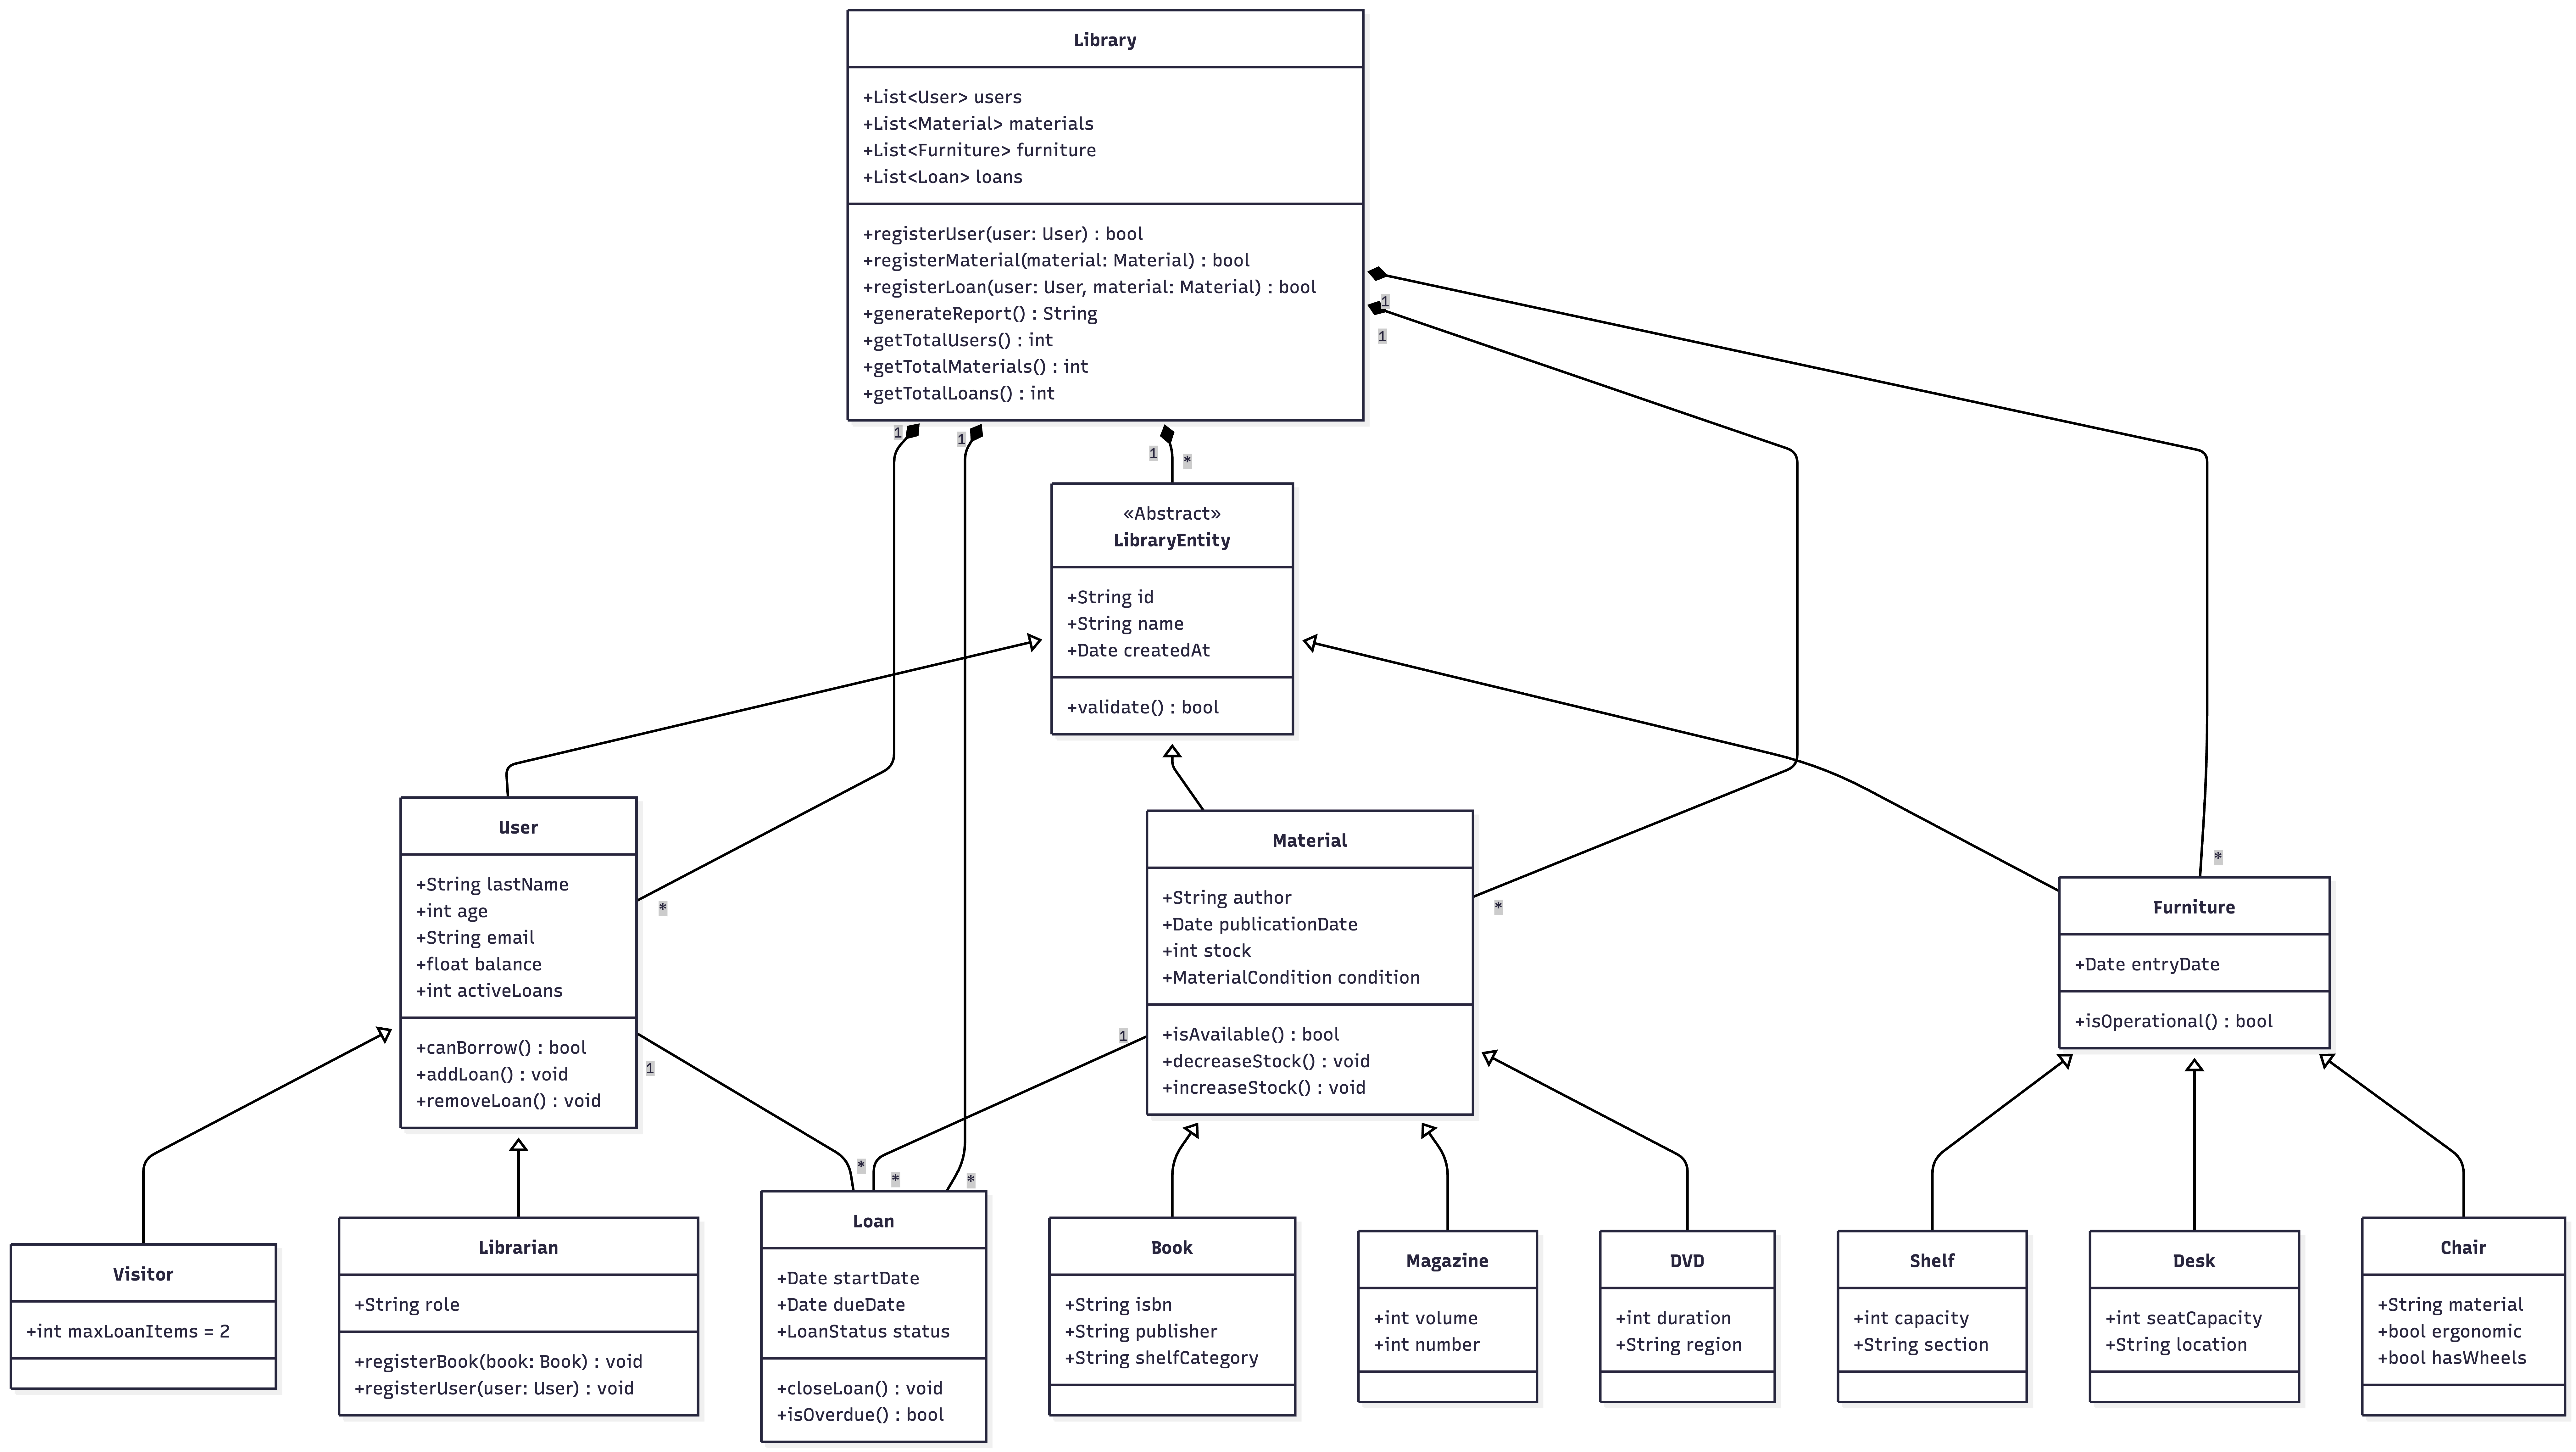
\includegraphics[width=0.5\textwidth]{attachtments/diagramaClaseUML.png}
        \captionof{figure}{Diagrama de Clase UML de sistema Biblioteca}
    \end{center}
    

    \section{Consideración de Requisitos No Funcionales}
    Para garantizar la calidad y viabilidad del sistema, se han priorizado los siguientes atributos:
    \begin{itemize}
        \item \textbf{Usabilidad}: El diseño debe ser intuitivo para facilitar su operación por parte del usuario final.
        \item \textbf{Robustez}: El sistema debe manejar adecuadamente los errores y excepciones para evitar interrupciones críticas.
    \end{itemize}

    % Descomenta las siguientes líneas si necesitas bibliografía
    % \newpage
    % \printbibliography

\end{document}
